\documentclass[../main.tex]{subfiles}
 
\begin{document}

% overview of the section

To better understand this research, one must understand basic information about \aclp{can}, about deep learning, and about related research. This section provides this background information. Specifically, Section \ref{sec:background:can} discusses the \acl{can}, including its message structure and contents. Section \ref{sec:background:dl} discusses time series classification approaches in deep learning and how they relate to this research. Section \ref{sec:background:related} discusses related work in \ac{can} analysis and fingerprinting vehicles, both with and without deep learning.

\subsection{The Controller Area Network}\label{sec:background:can}

The \acl{can} is a message broadcast system developed for automobile applications by Bosch in the early 1980s. The \ac{can} broadcasts short messages detailing the vehicle's functionality (e.g., wheel speed, engine temperature, velocity); this ensures data consistency throughout the vehicle. As Figure \ref{diagram:can-wiring} shows, this also reduces required wiring \cite{National-Instruments}.

\begin{figure}
    \centerline{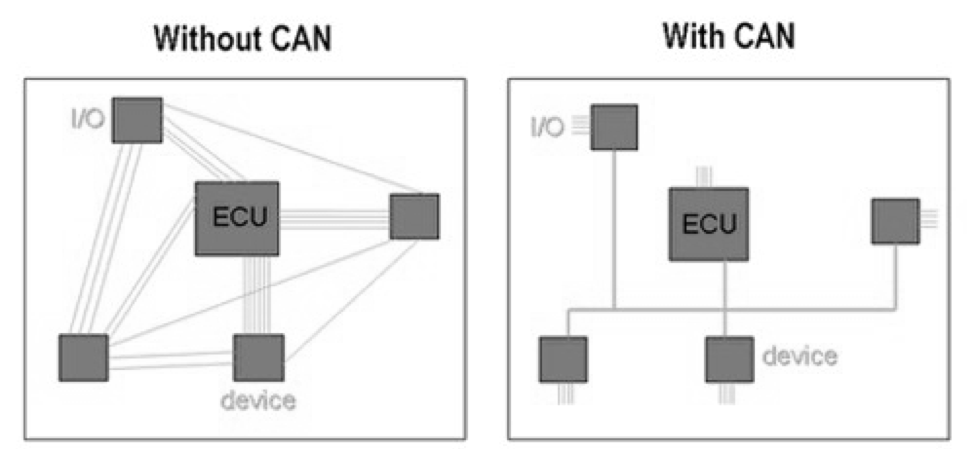
\includegraphics[scale=0.5]{can-wiring.png}}
    \caption{Vehicle network wiring with and without \ac{can}}
    \label{diagram:can-wiring}
\end{figure}

\ac{can} messages are limited in capacity: each one contains message overhead---including an arbitration ID, which identifies the message's contents to the network---and up to 64 bits of data \cite{Bosch1991, TexasInstruments2002}. Additionally, the components along the \ac{can} do not possess a wealth of computing power, so computational capabilities are also limited. For this reason, automobile manufacturers typically employ \textit{security through obscurity}, in which the exact data contents are obfuscated to prevent significant analysis. For example, it is difficult for a non-insider to learn what information is contained in messages with arbitration ID 704, even after significant reverse engineering efforts \cite{Buttigieg2017, Stone2018}. 

These obfuscation processes do not mask the vehicle itself: \ac{can} messages from one vehicle are uniquely identifiable. As this research shows, an attacker can devise a system capable of distinguishing \ac{can} messages from different vehicles. Such a system does not require massive data troves, and such a system is not limited by the \ac{can}'s low computational power. 

\subsection{Deep Learning}\label{sec:background:dl}

The \acl{mlp} is a feedforward neural network, which means that information flows from the input layer, through each hidden layer, and to the output layer \cite{Goodfellow2016}. \acp{mlp} are often called vanilla neural networks because they are simple, no-frills networks; one can use an \ac{mlp} to approximate a nonlinear function using few hidden layers \cite{Burkov2019}. In this research, we implement an \ac{mlp} to demonstrate an ability to classify \ac{can} data segments.

In deep learning, \aclp{cnn} ``are a specialized kind of neural network for processing data that has a known grid-like topology''; thus, these networks are well-suited for time-series data segments, which are effectively one-dimensional grids \cite{Goodfellow2016, Box1994}. By concatenating all sequential \ac{can} messages with the same arbitration ID, we obtain some unknown number\footnotemark[1] of time series. We then tune a \ac{cnn} to demonstrate its superior performance (as compared to an \ac{mlp}) when classifying \ac{can} data segments.

\footnotetext[1]{It is difficult to determine exactly how many unique signals are described by a single arbitration ID.}

\subsection{Related Work}\label{sec:background:related}

% identify and discuss references found, indicate that the paper is well informed, show where to find more info, see what prior work I rely on, see why the research is necessary, ensure prior work is organized by themes/messages

As discussed in \cite{Box1994}, most researchers concerned with time series data attempt to predict future values, especially those researchers focused on \ac{can} security. For example, \cite{Marchetti2017} devises an \ac{ids} by analyzing sequential \ac{can} IDs, and \cite{Tyree2018} creates an \ac{ids} that learns relationships in different time series signals. However, some researchers in recent years have used deep learning to classify \ac{can} data. For example, \cite{Kang2016} train a deep neural network to classify \ac{can} data packets as either \textit{normal} or \textit{abnormal}. The literature survey in \cite{Kwon2017} details more examples of deep learning as applied to \acp{ids} and \ac{can} security.

Recent research shows that one can certainly distinguish \ac{can} data. The researchers in \cite{Enev2016}, for example, demonstrate that machine learning can effectively discriminate between different drivers using just the reverse-engineered \ac{can} data collected from the vehicle. However, this research uses a set number of drivers, and it does not claim to distinguish raw time series generated by different vehicles.

% summary/transition paragraph

Clearly, various research efforts a) predict \ac{can} data but do not classify it, b) classify vehicles by analyzing reverse-engineered signals, or c) classify \ac{can} signals as good or bad. None of these efforts demonstrate an ability to classify vehicles using \textit{raw} \ac{can} data. This is an important gap in current research, and this research seeks to address this gap.

In the following section, we detail the experimental methodology, including the data's origins and structure and the data-formatting process. Additionally, we describe the deep learning models (i.e., their architectures and hyperparameters) and the model evaluation strategy.

\end{document}
